
	
		
		\paragraph{QuizziPedia::Front-End::AppRun}
		
		\label{QuizziPedia::Front-End::AppRun}
		
		\begin{figure}[ht]
			\centering
			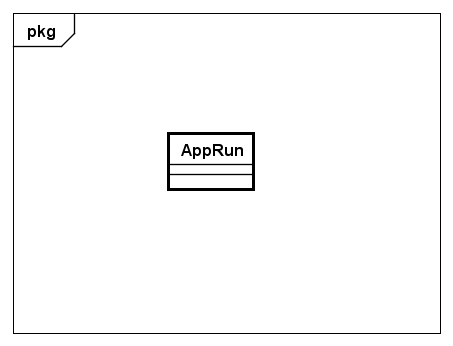
\includegraphics[scale=0.5,keepaspectratio]{UML/Classi/Front-End/QuizziPedia_Front-end_AppRun.png}
			\caption{QuizziPedia::Front-End::AppRun}
		\end{figure} \FloatBarrier
		
		\begin{itemize}
			\item \textbf{Descrizione}: classe che verifica se l'utente sia autenticato e che abbia le giuste autorizzazioni per la pagina in cui si trova;
			\item \textbf{Utilizzo}: viene utilizzata per verificare che l’utente sia autenticato e che abbia la giusta autorizzazione per la pagina in cui si trova;
			\item \textbf{Relazioni con altre classi}: 
			\begin{itemize}
				\item \textit{IN} \texttt{}: ; 
			\end{itemize}
			\item \textbf{Attributi}: 
			\begin{itemize}
				\item ;
			\end{itemize}
			\item \textbf{Metodi}: 
			\begin{itemize}
				\item ;
			\end{itemize}
		\end{itemize}
		